\documentclass[9pt]{IEEEtran}

\usepackage[english]{babel}
\usepackage{graphicx}
\usepackage{epstopdf}
\usepackage{fancyhdr}
\usepackage{tikz}
\usepackage{amsmath}
\usepackage{amsthm}
\usepackage{amssymb}
\usepackage{url}
\usepackage{array}
\usepackage{textcomp}
\usepackage{listings}
\usepackage{hyperref}
\usepackage{xcolor}
\usepackage{colortbl}
\usepackage{float}
\usepackage{gensymb}
\usepackage{longtable}
\usepackage{supertabular}
\usepackage{multicol}
\usepackage[utf8x]{inputenc}
\usepackage{csquotes}
\usepackage[backend=biber, style=numeric]{biblatex}
\addbibresource{bibliography.bib}
\usepackage[T1]{fontenc}
\usepackage{lmodern}
\input{glyphtounicode}
\pdfgentounicode=1
\graphicspath{{./figures/}}
\DeclareGraphicsExtensions{.pdf,.png,.jpg,.eps}

% correct bad hyphenation here
\hyphenation{op-tical net-works semi-conduc-tor trig-gs}

% ============================================================================================

\title{\vspace{0ex}
Modeling Social Distancing with Reinforcement Learning}

\author{Nejc Ločičnik, Igor Nikolaj Sok, Leon Todorov, Andraž Zrimšek \vspace{-4.0ex}}

% ============================================================================================
\addbibresource{literature.bib}
\begin{document}

\maketitle

\noindent\textit{\textbf{ABSTRACT: This study explores the use of reinforcement learning (RL) to model social distancing behaviors in artificial agents, aiming to minimize disease transmission in a two-dimensional environment. Inspired by natural behaviors observed in species like ants, agents exchange health information and adapt their movements to avoid infected individuals. We investigate how different reward structures, such as collision-based penalties and external tasks like wall-touching, influence agent behavior and the emergence of social distancing. Results show that agents trained with RL exhibited increased separation between healthy and infected agents, reducing infection spread. The findings suggest that RL can be a powerful tool for simulating disease dynamics and informing swarm robotics and public health strategies.}}

\section{Introduction}

The spread of infectious diseases presents a significant challenge to both human and animal populations, prompting the development of mechanisms to minimize transmission. Social distancing, an adaptive behavior where organisms avoid infected individuals, has been observed across various species, providing an evolutionary advantage in disease mitigation. During the COVID-19 pandemic, social distancing became a key public health strategy, prompting interest in how such behaviors might emerge in artificial agents.

Modeling disease transmission and social distancing behaviors in simulated environments can provide valuable insights for fields like epidemiology, robotics, and swarm intelligence. Traditional methods often rely on predefined rules, limiting the complexity and adaptability of agent behaviors. Reinforcement learning (RL), however, offers a flexible framework where agents learn to adapt based on reward structures, fostering more organic behaviors that evolve in response to environmental pressures.

In this study, we use RL to model social distancing behaviors in agents within a two-dimensional environment. By adapting their interactions based on health information exchanged with one another, agents aim to minimize disease transmission. Building on predator-prey dynamics in multi-agent RL frameworks, we explore how different reward structures and network adaptations contribute to the emergence of social distancing, where agents autonomously avoid infected individuals.

Our goal is to deepen the understanding of social distancing behaviors in adaptive multi-agent systems, with potential applications in disease transmission modeling, swarm robotics, and public health simulations.

\section{Related Work}

In Predator–prey survival pressure is sufficient to evolve swarming behaviors \cite{li2023predator}, the authors use reinforcement learning (RL) to model predator-prey dynamics in a cooperative–competitive multi-agent framework. Predators are rewarded for catching prey, and prey for avoiding capture, allowing agents to develop adaptive behaviors such as swarming and predator dispersion. Unlike traditional rule-based models, RL enables emergent, flexible behaviors that better reflect real-world complexity. Drawing from this, we adapt RL methods to model disease spread, tuning agent parameters and rewards to simulate social distancing behaviors.

Social distancing as a natural response to disease is further explored in Infectious diseases and social distancing in nature \cite{stockmaier2021infectious}, which examines how animals instinctively adjust interactions to reduce transmission. These behaviors arise through precautionary actions by healthy individuals or physiological responses in infected ones. Meanwhile, Romano et al. \cite{romano2022tradeoff}, in The trade-off between information and pathogen transmission in animal societies, highlight the balance between minimizing infection risk and maintaining critical social connections. They propose “network plasticity” as a mechanism enabling populations to optimize this trade-off, offering insights into decision-making within social groups.

Together, these studies provide frameworks for modeling adaptive behaviors under environmental pressures. Leveraging these insights, we use RL to simulate the dynamics of disease transmission, focusing on how agent interactions influence social distancing and infection spread.

\section{Methodology}

\subsection{Problem Definition}

Our objective is to simulate the spread of infectious diseases within a population of agents navigating a two-dimensional environment. The goal is to explore how agents can autonomously learn to minimize transmission by adapting their interactions based on health information exchanged with others. By aligning agent behavior with health-driven rewards and penalties, we aim to model emergent social distancing behaviors that limit contact with infected peers while balancing the need for interaction.

\subsection{Simulation Environment}

This study employs a multi-agent reinforcement learning (RL) framework, adapted from the environment developed by Li et al. (2023) \cite{li2023predator}. The simulation takes place in a two-dimensional continuous space with periodic boundary conditions, meaning that agents crossing one edge of the square environment reappear on the opposite edge, retaining their velocity.

Agents are modeled to resemble ants (changed from unicycles like in Figure \ref{fig:main_figure}), with their body consisting of three connected circles (the back circle being slightly larger) and six legs. Their behavior is driven by a combination of active and passive forces. Active forces, controlled by the agents, include a forward movement force ($aF$) aligned with their heading direction and a rotational force ($aR$) enabling changes in heading. Passive forces, inherent to the environment, include drag force ($Fd$), simulating resistance opposing the agent's velocity, and repulsive force ($Fa$), which prevents agents from overlapping by pushing them apart. At each simulation step, the agents' positions and velocities are updated by summing all acting forces, with the dynamics governed by:

$$ \dot{x} = v, \quad \dot{v} = \frac{ha_F + F_d + F_a}{m}, \quad \dot{\theta} = a_R $$  

where $x$ is the agent's position, $v$ its velocity, $\theta$ its heading angle, $h$ the unit vector for heading direction, and $m$ the agent's mass. The agents along with the forces acting on them are illustrated in Figure \ref{fig:main_figure}.

\begin{figure}[hbt]
    \centering
    \begin{minipage}{0.2\textwidth}
        \centering
        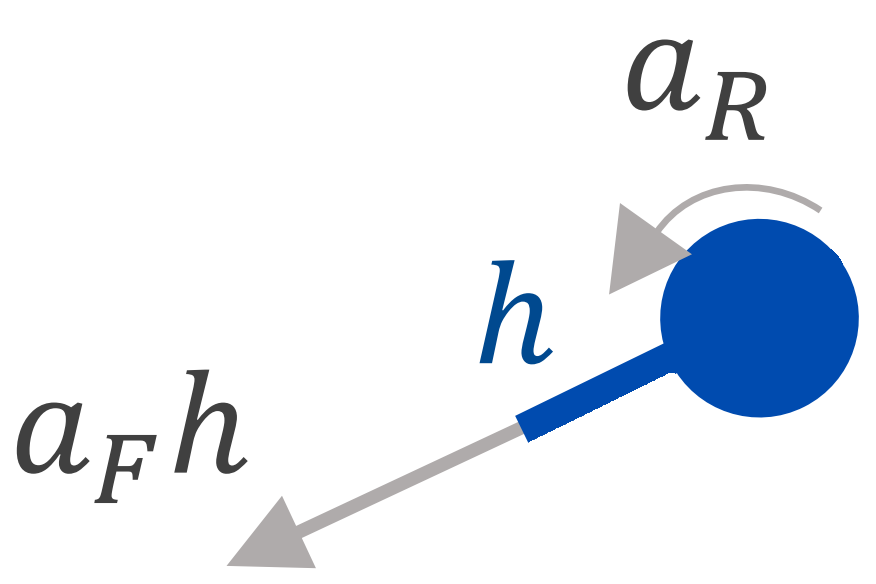
\includegraphics[width=\textwidth]{agent_active.png}
        %\caption{Active forces.}
        %\label{fig:image1}
    \end{minipage}
    \hspace{0.1cm}
    \begin{minipage}{0.25\textwidth}
        \centering
        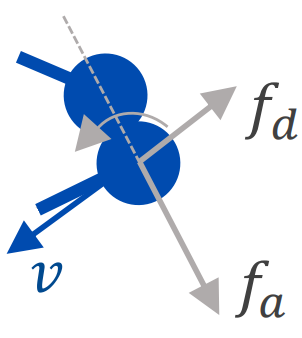
\includegraphics[width=\textwidth]{agent_passive.png}
        %\caption{Passive forces.}
        %\label{fig:image2}
    \end{minipage}
    \caption{Active (left) and passive (right) agent forces. \cite{li2023predator}}
    \label{fig:main_figure}
\end{figure}

To tailor the framework to our objectives, we implemented several modifications: 1) changed agent visualization from unicycles to ant-like figures and adjusted movement parameters; 2) incorporated health status perception for each agent; 3) tracked agent interactions for network evaluation; and 4) redefined the reward policy to align with disease-spread mitigation goals.

\subsection{Basic Reward Policy}

Our initial reward policy aimed to produce social distancing patterns in agent behavior is based on direct collisions between agents as the primary form of information exchange. Collisions between agents of the same status (healthy-healthy or infected-infected) were rewarded to encourage grouping behavior. In contrast, collisions between agents of different statuses (healthy-infected or vice versa) were penalized to discourage close contact to limit disease spread.

The above mention policy is demonstrated in isolation with all healthy agents in Figure \ref{fig:demo}. On the left simulation we penalized each agent upon collision with a $-1$ reward, while on the right simulation we rewarded each colliding agent with a $+1$ reward. This demonstrates how a very simple change in the reward policy effects the learned behavior.

\begin{figure}[hbt]
    \centering
    \begin{minipage}{0.2\textwidth}
        \centering
        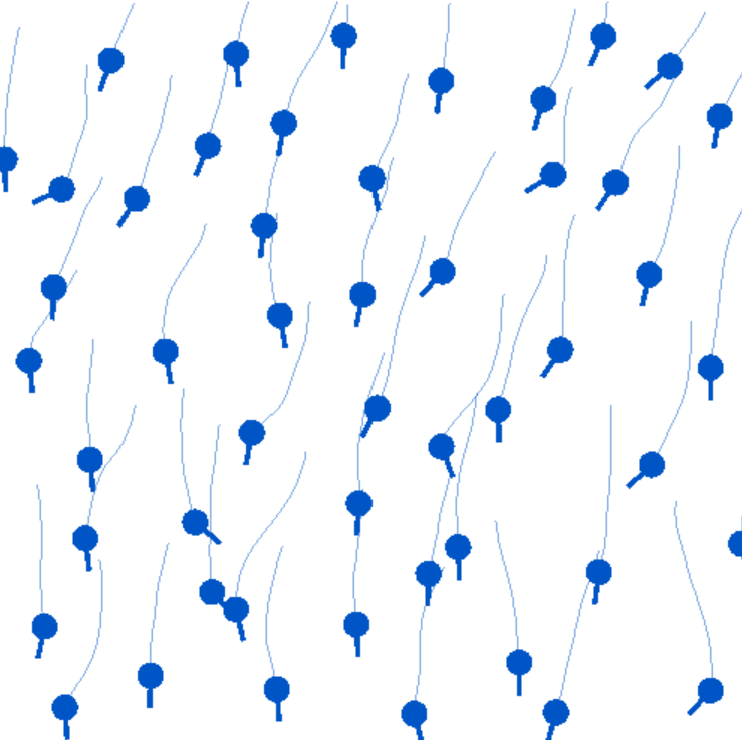
\includegraphics[width=\textwidth]{avoid.png}
    \end{minipage}
    \hspace{0.5cm}
    \begin{minipage}{0.2\textwidth}
        \centering
        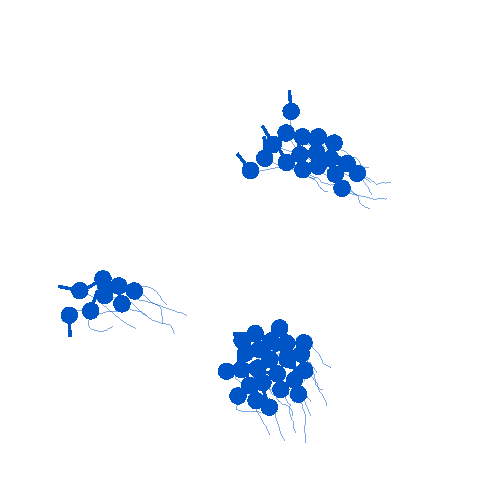
\includegraphics[width=\textwidth]{touch.png}
    \end{minipage}
    \caption{Demonstration of simple reward policies - penalize (left) or reward (right) collisions.}
    \label{fig:demo}
\end{figure}

We tried a few approaches to augment the simple reward policy:

\begin{enumerate} 
    \item \textbf{Diminishing Reward for Interactions} $\rightarrow$ To reduce agent clustering, consecutive interactions were progressively penalized based on recent interactions ($h(x)\rightarrow$ health status of agent $x$).
$$
\mathrm{reward}(a, b) = \begin{cases}
    -\lambda & \text{if } h(a) \neq h(b) \\ 
    +\sigma * \gamma (1 - recent(a,b)) & \text{otherwise.}
\end{cases}
$$
    \item \textbf{Wall Collision Penalty} $\rightarrow$ In non-periodic environments, we penalized agents for colliding with walls. 
$$
\mathrm{reward}(a) = \begin{cases}
    -\lambda & \text{if a collides with any wall}\\ 
    0 & \text{otherwise.}
\end{cases}
$$
    \item \textbf{Energy Control Penalty} $\rightarrow$ A control penalty was introduced to simulate energy consumption, penalizing the magnitude of the agent’s control inputs.
$$
\text{reward}(aF, aR) = -(\alpha |aF| + \beta |aR|)
$$
\end{enumerate}

However, we found these approaches too engineered for our goals and ultimately decided to stick with a simpler reward policy.

What we did find to vastly improve visualization results was the introduction of an external task. This task added complexity that better reflected real-world dynamics. Agents alternated between touching the left and right walls, with each agent initially assigned a wall. They were rewarded $+0.1$ for moving in the correct direction and $+1$ for reaching the assigned wall. After completing the task, agents switched to the opposite wall, requiring them to continuously adapt their movement strategy. This task significantly enhanced the agents' performance and provided clearer insights into their behavior.

\subsection{Alternative Information Exchange}

Our main exploration of agent interaction (information exchange) was on the basis of collisions. As an alternative, we also considered a pheromone-based system inspired by ant behavior, where agents perceived "safety" or "danger" through accumulated, decaying concentrations. While promising in theory, this approach performed poorly compared to integrating movement-based tasks. The core issue was the lack of a clear relationship between pheromone observations and the actions needed to maximize rewards. This underscores the importance of designing observation mechanisms that directly guide actionable, reward-driven behavior.

\section{Results}

\subsection{Interaction Network Observations}

To assess the emergence of social distancing behaviors, we convert agent interactions into a network as described in Stroeymeyt et al. (2018) \cite{Stroeymeyt2018}. During each evaluation step, interactions are recorded in an $n \times n$ matrix, where $n$ is the total number of agents. A collision between agents is considered an interaction. After each evaluation, the matrix is normalized to create the network, where nodes represent agents and edges form if interaction values exceed a $0.01$ threshold. Edge weights correspond to interaction values, and nodes are labeled with the agents' health status.

We evaluated our trained model over a $10,000$-step episode using both a random, untrained network and a trained network, constructing interaction networks to analyze agent behavior. The random network lacked structure, forming a mostly fully connected graph. In contrast, the trained network exhibited separation, with infected agents interacting less with healthy ones while maintaining interactions with other infected agents. When edges were weighted by interaction frequency, these patterns became clearer, as shown in Figure \ref{fig:filtered_net}.

\begin{figure}[hbt]
    \centering
    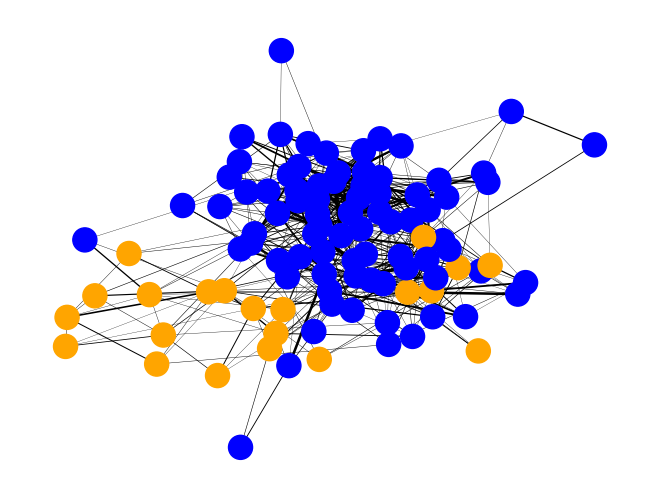
\includegraphics[width=0.9\linewidth]{filteredNet.png}
    \caption{Filtered learned interaction network.}
    \label{fig:filtered_net}
\end{figure}

We calculated network metrics such as clustering, modularity, and density to quantify agent interactions. Modularity increased from $-0.0005$ (random) to $0.25$ (trained), and clustering rose from $0.056$ to $0.066$, indicating greater group separation and the emergence of social distancing. These changes align with reduced infection spread, as suggested in \cite{volz2011effects}.

To study pathogen-induced changes, we ran $10$ experiments using the best-performing model. In each, agents were designated as infected, and a baseline $10,000$-step evaluation was conducted without actual infections. Metrics were recorded before and after introducing infections. Results in Figure \ref{fig:induced_changes} show increased modularity as infected agents segregated and decreased network efficiency, consistent with reduced pathogen spread. However, clustering unexpectedly decreased due to the high connectivity of the initial infection-free network, where agents formed dense groups with a clustering coefficient of $0.138$.

\begin{figure}[hbt]
    \centering
    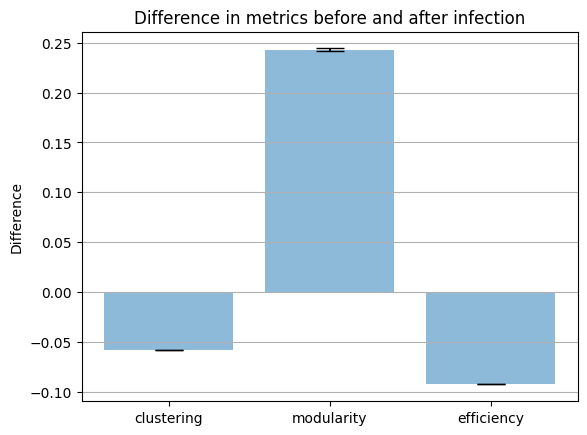
\includegraphics[width=0.9\linewidth]{figures/induced_changes.png}
    \caption{Changes in interaction network properties when introducing infected agents.}
    \label{fig:induced_changes}
\end{figure}

The results, shown in Figure \ref{fig:induced_changes}, reveal a significant increase in modularity, as infected agents became more segregated from the healthy population. Additionally, network efficiency decreased, suggesting an increase in the shortest paths within the network, which is consistent with reduced pathogen spread. However, contrary to expectations, clustering decreased. This anomaly can be explained by the initial lack of infected agents, resulting in a highly connected network with a high clustering coefficient of $0.138$ due to the agents’ tendency to form dense groups.

\subsection{Simulation Visualization Observations}

\begin{figure}[hbt]
    \centering
    \begin{minipage}{0.2\textwidth}
        \centering
        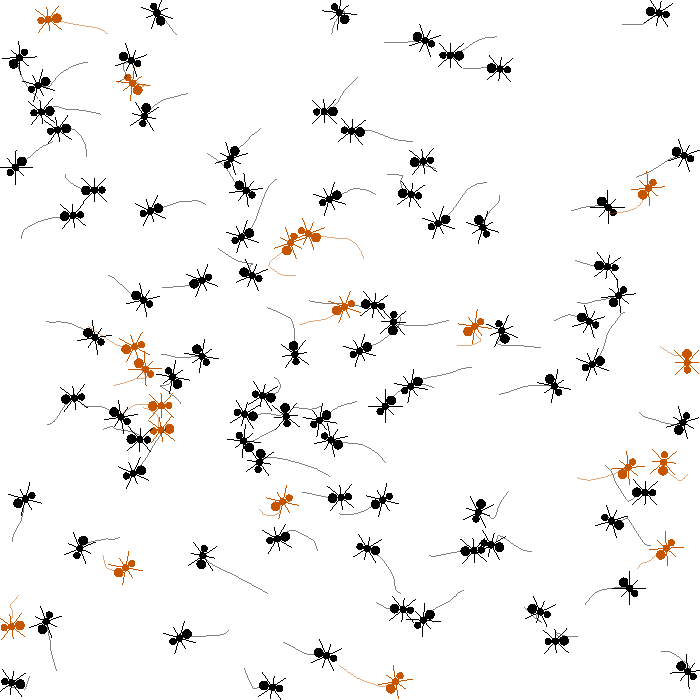
\includegraphics[width=.9\linewidth]{frame_25.png}
    \end{minipage}
    \hspace{0.2cm}
    \begin{minipage}{0.2\textwidth}
        \centering
        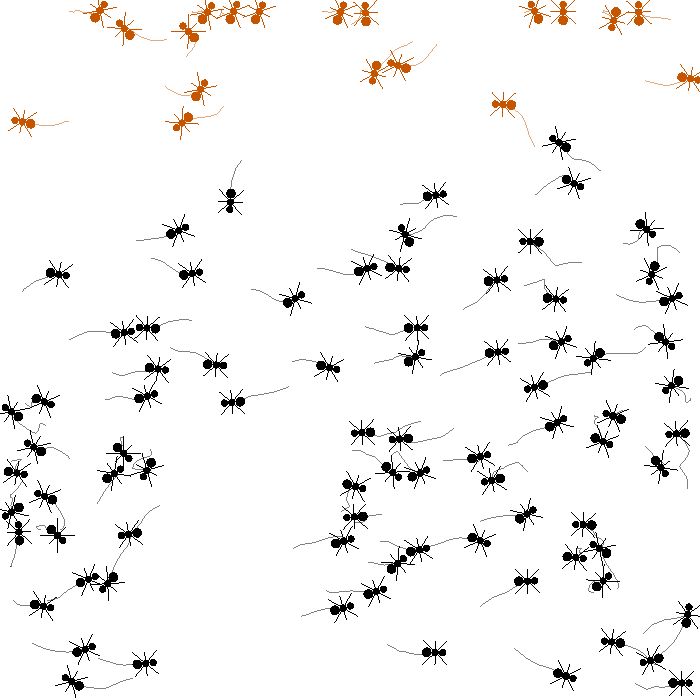
\includegraphics[width=.9\linewidth]{frame_1300.png}
    \end{minipage}
    \caption{Start of simulation (left) compared to end of simulation (right)}
    \label{fig:trained_viz}
\end{figure}

Figure \ref{fig:trained_viz} illustrates a simulation of our best-performing policy. Orange ants represent infected agents, while black ants represent healthy ones. The left image (frame $25$) shows the start of the simulation, and the right image (frame $1300$) depicts a later stage. A clear separation between the two groups is observed, minimizing contact between agents of different health statuses. Notably, this separation only emerged after introducing the additional left-to-right movement task. Without this task, while the interaction network properties remained similar, the visual separation was far less pronounced.

\section{Discussion}

This study used reinforcement learning (RL) to model social distancing behaviors in artificial agents, aiming to minimize disease transmission in a two-dimensional environment. Inspired by natural behaviors like those of ants, agents exchanged health information and adapted their movements to avoid infected individuals, simulating social distancing.

Results showed that agents trained with a basic reward policy increased the separation between healthy and infected agents, as reflected in network metrics like modularity and clustering. These metrics indicated that agents successfully minimized disease transmission by avoiding contact with infected individuals.

We also examined the impact of reward components, including diminishing rewards, control penalties, and wall collision penalties, which refined agent behavior and encouraged more efficient movement patterns. Additionally, agents alternated between touching walls, promoting more structured behavior and facilitating social distancing. In contrast, a pheromone-based exchange system was less effective due to its misalignment with reward-driven actions.

Our findings suggest RL can effectively model disease spread and social distancing behaviors. Future research could build on these results by incorporating more complex disease dynamics, improving agent interactions, and applying the model to public health simulations and swarm robotics.
\\

\noindent\textbf{CONTRIBUTIONS}: \textbf{LT} prepared/fixed the environment setup and did the basic avoid/touch experiments, \textbf{INS} and \textbf{AZ} did the reward policy experiments and the network statistics, \textbf{NL} did the alternative interactions experiment and organized/polished the report. Each member wrote their own parts of the report.

\printbibliography

\end{document}
